
\section{Sistemi termici}
Al fine di descrivere i sistemi termici è fondamentale conoscere l'equazione
del bilancio termico.

Si considera un certo volume di superficie $S$ caratterizzato da un unico
parametro: la \textit{capacità termica}; la capacità termica di un corpo è
l'attitudine del corpo a modificare la sua temperatura quando questo viene
investito da una certa potenza termica.

È inoltre esprimibile come il rapporto tra il calore entrante nel corpo e la
variazione di temperatura che esso subisce, è considerata un'inerzia termica.
Il volume può interagire con l'ambiente che lo circonda mediante la superficie
$S$, quest'ultima consente di realizzare gli scambi di potenza termica.
%Posizione della figure non specificata, [h] missing
% è una prova dell'impaginamento automatico di LaTex
\begin{figure}
 \centering
 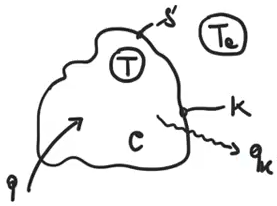
\includegraphics[width=\picwid]{corpo_termico.png}
 % corpo_termico.png: 277x206 px, 96dpi, 7.33x5.45 cm, bb=0 0 208 154
 \label{Fig.:corpo_termico}
\end{figure}

Si suppone inoltre che il corpo abbia una temperatura uniforme $T$, costante in
ogni suo punto, l'ambiente esterno invece sarà ad una temperatura $T_a\neq T$.

La differenza tra le due temperature genererà dei flussi di potenza termica dal
corpo (o ambiente) più caldo a quello più freddo.
La quantità di energia termica che attraversa la superficie dipenderà dalla
superficie stessa e in particolare dalla sua \textit{resistenza termica}.

Si indica con $K$ il coefficiente di scambio termico che la superficie consente
di sviluppare.
Il flusso termico $q_K$ è definito per convenzione positivo se uscente dal
corpo, dunque
$$
q_K = K(T-T_a)
$$

Si riportano le equazioni di bilancio termico che interessano il volume se
questo è sottoposto ad $n$ flussi termici $q_n$ ed $i$ superfici di scambio
termico con coefficiente di scambio $K_i$ e con ambienti a temperature $T_i$
(diverse o meno fra loro):
\begin{equation}
C\dot{T} = \sum_n q_n -\sum_i K_i(T-T_i)
\label{eq.:bilancio_termico}
\end{equation}

Si riporta il modello ISU del sistema in esame con una sola potenza termica in
ingresso ed un solo scambio termico con un unico ambiente
 a temperatura $T_a$
$$
C\dot{T} = q -K(T-T_a)
$$
variabili:
$$\begin{matrix}
q & T_a & T \\
(0) & (0) & (1) \\
u_1 & u_2 & x
\end{matrix}
$$
\emph{Attenzione, $T_a$ è a tutti gli effetti una variabile di ingresso, anche
se resta costante, si parla di ingresso non manipolabile}

Equazioni del sistema:
$$\left\{\begin{aligned}
\dot{x} &=  \dot{T} = \frac{1}{C}u_1-K(x-u_2) \\
y &= T = x
\end{aligned}\right.$$

\subsection{Esempio forno elettrico}
Dato un volume chiuso si indica con $C_1$ la sua capacità termica e $T_1$ la
sua temperatura.
Si suppone che sia presente attorno al volume una parete con capacità termica
$C_2$ ed una temperatura supposta uniforme $T_2$, l'ambiente esterno è alla
temperatura $T_a$.
All'interno del volume è presente una resistenza elettrica che fornisce una
certa potenza termica $q$.

\begin{figure}[h]
 \centering
 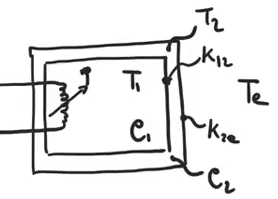
\includegraphics[width=\picwid]{forno_elettrico.png}
 % forno_elettrico.png: 278x199 px, 96dpi, 7.35x5.26 cm, bb=0 0 208 149
 \label{Fig.:forno_elettrico}
\end{figure}

Attraverso la parete, la temperatura è in realtà un gradiente termico e non
uniforme.
Si indicano con $K_{12}$ e $K_{2a}$ i coefficienti di scambio termico tra le
rispettive superfici.

Per ogni volume con una certa capacità termica, va scritta un'equazione del
bilancio
$$\left\{\begin{aligned}
C_1\dot T_1 &= q - K_{12}(T_1-T_2)\\
C_2\dot{T}_2 &= -K_{12}(T_2-T_1) - K_{2a}(T_2-T_a)
\end{aligned}\right.$$
Si nota come il flusso termico $K_{12}(T_1-T_2)$ uscente dal primo volume sia
entrante nel secondo.
Utilizzando sempre la stessa convenzione sui versi non si commettono errori e
non bisogna riflettere sui versi effettivo dei flussi termici.

Variabili:
$$\begin{matrix}
q & T_a & T_1 & T_2 \\
(0) & (0) & (1) & (1) \\
u_1 & u_2 & x_1 & x_2
\end{matrix}$$
Il sistema è di ordine due.

$$\left\{\begin{aligned}
\dot x_1 &= \dot{T}_1 = \frac{1}{C_1}u_1 - K_{12}(x_1-x_2)\\
\dot x_2 &= \dot T_2 = -\frac{K_{12}}{C_2} (x_2-x_1) -
\frac{K_{2a}}{C_2}(x_2-u_2)\\
y_1 &= T_1 = x_1 \\
y_2 &= T_2 = x_2
\end{aligned}\right.$$

Se si indica con $v$ la tensione ai capi della resistenza $R$, la potenza
termica si sarebbe potuta esprimere come $q=\frac{v^2}{R}$ e se si fosse scelta
$v$ come ingresso si avrebbe avuto un termine al quadrato
$$
\dot x_1 = \dot T_1 = \frac{1}{C_1 R} u_1^2 - K_{12}(x_1-x_2) \dots
$$
Lo stesso sistema, con variabili diverse sarebbe diventato non lineare.

\section{Sistemi idraulici}
Un sistema idraulico è modellabile come un serbatoio in grado di contenere un
certo liquido. Si suppone che ci sia la possibilità di aggiungere una certa
quantità di liquido $q_i$.

Si suppone che la sezione del serbatoio sia regolare ed $h$ l'altezza del
liquido nel serbatoio. Si suppone che sia presente una valvola in uscita in
grado di prelevare un flusso di liquido in uscita $q_u$, analogamente con una
valvola in ingresso.

\begin{figure}[h]
 \centering
 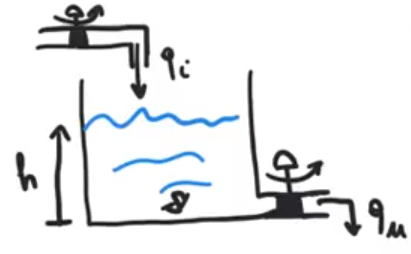
\includegraphics[width=\picwid]{serbatoio_due_valvole.png}
 % serbatoio_due_valvole.png: 411x254 px, 96dpi, 10.87x6.72 cm, bb=0 0 308 190
 \label{Fig.:serbatoio_due_valvole}
\end{figure}


Il flusso di un liquido viene chiamato \textbf{portata} e ci si può
riferire
ad una portata \textit{massica} ($w$) [\si{\kilogram/\second}]
 o \textit{volumetrica} ($q$) $\si{\meter^3/\second}$, con la seguente
relazione che le lega
$$
w = \rho q
$$
dove $\rho$ è la \textit{densità} del liquido.

È fondamentale considerare i liquidi incomprimibili, ossia che la sua densità
resti costante affinché si possa sempre utilizzare l'uno o l'altro riferimento.
Ci si riferirà generalmente alla portata volumetrica.

La quantità di massa nel serbatoio è pari alla differenza di massa entrante e
uscente, supposta la densità costante invece si può quindi ragionare sui volumi
e le $j$ portate entranti e $k$ portate uscenti ossia:
$$
\dot{V} = \frac{d}{dt}(S\cdot h) = S\dot{h} = \sum_j q_i - \sum_k q_u
$$
con $\dot{V}$ la variazione di volume e $S$ la sezione del serbatoio
assunta costante (altrimenti $S\dot h + \dot{S}h$).

Per il sistema in esame con un ingresso ed un'uscita si ha
$$
\dot{V} = q_i - q_u
$$
Si suppone che la valvola in uscita sia autoregolata, la portata di un fluido
attraverso una valvola dipende sia dalla sua sezione regolabile che dalla
differenza di pressione a monte e a valle della stessa, funzione dell'altezza
del fluido.

Un modello semplice di valvola ammette un parametro $a$ che
indica il grado di apertura della valvola ed esprime la portata con la
seguente
$$
q = a\sqrt{h}
$$

Si scrive il modello ISU, l'equazione è già stata ricavata, si procede con le
variabili:
$$
\begin{matrix}
q_i & h \\
(0) & (1) \\
u & x
\end{matrix}
$$

$$\left\{\begin{aligned}
\dot{x} &= \dot{h} = \frac{1}{S} u - \frac{a}{S}\sqrt{x} \\
y &= V = Sh = Sx
\end{aligned}\right.$$
Il sistema è non lineare e strettamente proprio.

\subsection{Sistema idraulico con due serbatoi}
Si ha un sistema formato da due serbatoi in cascata con un flusso
monodirezionale tra l'uscita di uno e l'ingresso dell'altro.
\begin{figure}[h]
 \centering
 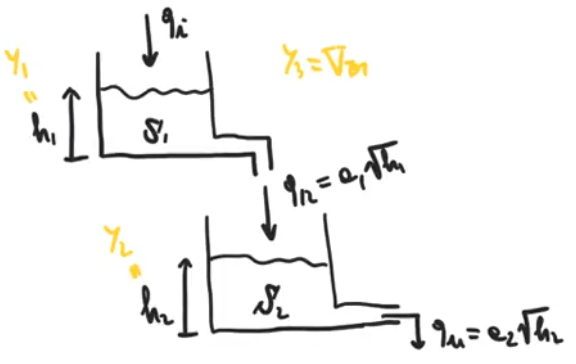
\includegraphics[width=\picwid]{doppio_serbatoio.png}
 % doppio_serbatoio.png: 576x364 px, 96dpi, 15.24x9.63 cm, bb=0 0 432 273
 \label{Fig.:doppio_serbatoio}
\end{figure}

Si indica con $h_1$ l'altezza di liquido nel serbatoio di sezione $S_1$ ed
$h_2$ l'altezza nel serbatoio di sezione $S_2$. Le portate in uscita dai due
serbatoi saranno:
$$\begin{aligned}
q_{12} &= a_1\sqrt{h_1} //
q_u &= a_2\sqrt{h_2}
\end{aligned}$$

Le equazioni del sistema saranno:
$$\left\{\begin{aligned}
S_1\dot h_1 &= q_i - q_{12} = q_i - a_1\sqrt{h_1} \\
S_2 \dot h_2 &= q_{12} - q_u = a_1\sqrt{h_1} - a_2\sqrt{h_2}
\end{aligned}\right.$$

Si analizzano le variabili
$$\begin{matrix}
q_i & h_1 & h_2 \\
(0) & (1) & (1) \\
u & x_1 & x_2
\end{matrix}$$

Il sistema di ordine due in forma ISU
$$\left\{\begin{aligned}
\dot x_1 &= \dot h_1 = \frac{1}{S_1} u - \frac{a_1}{S_1} \sqrt{x_1} \\
\dot x_2 &= \dot h_2 = \frac{a_1}{S_2}\sqrt{x_1} - \frac{a_2}{S_2} \sqrt{x_2} \\
y_1 &= h_1 = x_1 \\
y_2 &= h_2 =x_2 \\
y_3 &= V_{\text{tot}} = S_1h_1 + S_2h_2 = S_1x_1 + S_2 x_2
\end{aligned}\right.$$

Il sistema è non lineare strettamente proprio.

Se il legame tra la portata e l'altezza fosse lineare, il sistema diventerebbe
lineare, può essere sensato linearizzare la funzione in particolari regimi di
funzionamento della valvola.


\section{Equilibrio dei sistemi}
Si ricordi il modello generale di un sistema ISU presentato con la
\ref{eq.:ISU_generale}
$$
\left\{\begin{aligned}
\dot x & = f(x,u,t) \\
y &= g(x,u,t)
\end{aligned}\right.
$$
non è nota l'espressione della $x(t)$, andrebbe
integrato il sistema di equazioni, non è detto che sia possibile; se la
funzione $f$ è lineare e tempo invariante è possibile integrare, se il sistema
non è invece lineare non è detto che sia possibile risolverlo in forma chiusa.

Si supponga che i sistemi godano almeno della proprietà di tempo invarianza
(coefficienti costanti) o di una lenta tempo varianza nei regimi operativi di
analisi.

Si danno le seguenti definizioni:
\begin{itemize}
\item \textbf{Movimento} nello stato del sistema: Assegnato un certo ingresso
ed una certa condizione iniziale, si definisce la soluzione del sistema in
esame per $t\geq t_0$
$$
\tilde{x}(t_0) ,\ \begin{aligned}[t]&\tilde{u}(t)\\ [&t_0, t]\end{aligned}
\longrightarrow \tilde x(t)\quad t\geq t_0
$$


Tra i possibili movimenti ce ne sono alcuni di particolari interesse

\item \textbf{Equilibrio}:

Dato un ingresso costante $\overline{u}$ esiste uno stato costante
$\overline{x}$ tale per cui la funzione di transizione $f$ calcolata sia pari a
zero.
$$
\overline{u} = \text{ cost} ,\ \exists\  \overline{x} = \text{ cost} \quad :
\quad f(\overline{x},\overline{u})=0 \Leftrightarrow \text{Equilibro}
$$
La tripletta $(\overline{u},\overline{x},\overline{y})$ viene definita punto di
\textbf{equilibrio del sistema}.

Se la funzione di transizione è nulla allora la $\dot x$ è nulla, dunque il
sistema non modifica il suo stato, lo stato perdura indefinitamente nel tempo,
dunque i punti di equilibrio sono movimenti costanti del sistema sottoposto ad
ingressi costanti.
Nella realtà nessun ingresso è mai costante.

Variando l'ingresso il sistema raggiunge un nuovo punto di equilibrio dopo un
certo transitorio, la maggior parte dei sistemi studiati lavorano in stati
costanti a tratti, mutano tra un punto di equilibrio e l'altro.
\end{itemize}

\subsection{Equilibrio del pendolo}
\label{sec.:equilibrio_del_pendolo}
Si riprende l'esempio del pendolo rigido analizzato alla sezione
\ref{sec.:pendolo_rigido}
\begin{figure}[h]
 \centering
 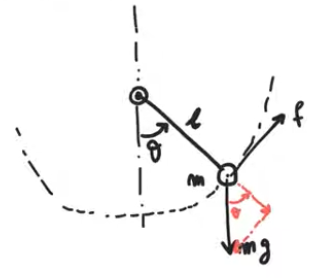
\includegraphics[width=\picwid]{pendolo.png}
 % pendolo.png: 316x278 px, 96dpi, 8.36x7.35 cm, bb=0 0 237 208
 %\label{Fig.:pendolo_semplice}
\end{figure}
Il sistema ha un punto di equilibrio?
Intuitivamente il punto di equilibrio è quello a $\theta=0$, in realtà anche
$\theta=\pi$ è un punto di equilibrio, in assenza della forza $f$ solo la forza
peso agisce sul sistema e in queste due posizioni è completamente bilanciata
dal vincolo dato che l'asta è rigida.

Se invece la forza $f$ applicata è diversa da zero e pari alla componente
tangente della forza peso $mg\sin(\theta)$ allora la condizione di equilibrio
si troverà in un punto diverso dai precedenti, inclinato di un certo angolo
$\theta$, e sarebbe in equilibrio anche nell'angolo $\pi - \theta$ rimanendo
fermo.

Il caso limite è quando l'asta diventa perfettamente orizzontale, il punto di
equilibrio diventa unico, $\theta = 90\text{\textdegree}$.

Se $f > mg$ il pendolo comincia a ruotare e non ci saranno più punti di
equilibrio.

Si riprende il modello analitico del pendolo ricavato in
\ref{eq.:pendolo_semplice}
$$
x_1 = \theta\ x_2 = \dot\theta\ u=f
$$
\begin{equation*}
\left\{\begin{aligned}
\dot x_1 &= \dot\theta = x_2 = f_1\\
\dot x_2 &= \ddot\theta = \frac{1}{mL} u - \frac{g}{L}  \sin(x_1) =f_2 \\
y &= \theta = x_1
\end{aligned}\right.
\end{equation*}

Il sistema ammette punti di equilibrio? Dalla definizione, se il sistema
ammette punti di equilibrio bisogna trovare una coppia
$(\overline{u},\overline{x})$ tali che la funzione di transizione $f$ sia pari
a zero.
$$
(\overline{u},\overline{x}) \Rightarrow f(\overline{u},\overline{x}) = 0
$$

Dunque si costruisce il sistema per ricavare lo stato di equilibrio
$$\left\{\begin{aligned}
&\overline{x}_2 = 0 \rightarrow \dot\theta = 0\\
&\frac{1}{m\cancel{L}} \overline{u} - \frac{g}{\cancel{L}}
\sin(\overline{x}_1)=0 \rightarrow \sin(\overline{x}_1) =
\frac{1}{mg}\overline{u}
\end{aligned}\right.$$
La velocità deve essere nulla e la soluzione è indipendente dalla lunghezza
dell'asta.

Analizzando la seconda equazione si ha che la funzione seno è limitata tra
$[-1,1]$ dunque
$$
\frac{|\overline{u}|}{mg} \leq 1 \Longleftrightarrow
|\overline{u}| \leq mg
$$

Le equazioni confermano quanto intuito precedentemente, la forza peso $mg$ deve
essere maggiore o uguale della forza $f$ applicata dall'esterno.

Si studiano i seguenti casi
$$|\overline{u}| \leq mg\left\langle
\begin{aligned}
& \\
&|\overline{u}|=mg \left\langle \begin{aligned}
&\overline{u} = mg \Rightarrow\sin(\overline{x}_1) = 1 \Rightarrow
\overline{x}_1 = \frac{\pi}{2}\\
&\overline{u} = -mg \Rightarrow \sin(\overline{x}_1) = -1 \Rightarrow
\overline{x}_1 = -\frac{\pi}{2}
\end{aligned}  \right.
& \\
& \\
&|\overline{u}|<mg \Rightarrow \overline{x}_1 = \left\langle \begin{aligned}
&\sin^{-1}\left(\frac{\pi}{mg}\right) \\
&\pi - \sin^{-1}\left(\frac{\pi}{mg}\right)
\end{aligned}\right.
&\\
& \\
\end{aligned}\right.
$$
Si è quantificato numericamente il valore degli angoli di equilibrio del
sistema.
